\chapter{使用该模版}

下面开始介绍如何使用这个模版,序言里已经提过,
这个模版的目的就是让没有一点\LaTeX 基础的同学也能很快地用\LaTeX 组织出自己的论文。
因此,这个模版没有过多的选项,只有一些和写Word同等难度\footnote{是的,难度少很多很多。这是一个测试用的脚注}的注意事项。
但难点,要比Word少很多。

这个模板一共需要如下几个文件:
\begin{enumerate}
\item{ZJUthesis.cls},这个是模版文件;
\item{ZJUthesis.cfg},这个是模版的配置文件,与模版文件配合使用;
\item{ZJUthesis.bst},这个是参考文献的格式说明文件;
\item{文件夹CoverPagepic},存放着封面使用到的浙大校名与校徽图片;
\item{CoverPagepic$\backslash$ZJDX.eps},eps\index{eps}格式\footnote{关于eps格式,
图片一节中将会做进一步介绍}的浙大校名图片;
\item{CoverPagepic$\backslash$ZJDX.pdf},pdf格式\footnote{同eps解释}的浙大校名图片;
\item{CoverPagepic$\backslash$QSY.eps},eps格式的校徽;
\item{CoverPagepic$\backslash$QSY.pdf},pdf格式的校徽。
\item{Chapter$\backslash$Copyright.tex},这个是版权转让声明。
\item{Signature$\backslash$sign\_ch.eps等七个签名文件},这个是作者签名,默认是一个空白的eps,提交最终版的时候可将其替换为相应的签名图片,直接可以作进pdf文档中去。这七个文件同样有其相对应的pdf格式图形文件,其文件名与相应签名对应如下:

{
\zihao{5}
\begin{tabular}{cl}
sign\_ch & 作者的中文签名(中文题名页用)\\
sign\_ch\_s & 导师的中文签名(中文题名页用)\\
sign\_en & 作者的英文签名(英文题名页用)\\
sign\_en\_s & 导师的英文签名(英文题名页用)\\
sign\_cr\_1 & 作者的中文签名(版权声明页用)\\
sign\_cr\_2 & 作者的中文签名(版权声明页用)\\
sign\_cr\_s & 导师的中文签名(版权声明页用)\\
\end{tabular}
}

当然,其中几个签名可以用同一个文件复制使用。也可以做七个不同的使用。
要注意的是签名的图形文件长宽比大约控制在2:1。
\end{enumerate}

现在即可以用winEdt或者其它习惯使用的文本编辑器,
打开这个文档的tex源文件,就是叫做“论文模版示例.tex”的这个文件。
我们书写论文,就是写这样一个扩展名为“tex”的纯文本文件。

我们现在开始它的第一行。

\section{模版选项}

%$\backslash$documentclass[oneside]\index{oneside}\{ZJUthesis\}
{\noindent\zihao{-5}\verb+\documentclass[oneside]{ZJUthesis}+}

这一句就指明了这个文档所用的格式模版,就是浙大的论文模版,{\bf ZJUthesis}
就是这个模版文件的文件名。
而{\bf$\backslash$documentclass}则是一个命令,在\LaTeX 源文件中,
以斜线$\backslash$开头的的字母字符串,都是一个命令,
命令只能由一个斜线及其引领的字符串构成,不能包含数字与其它符号,
当遇到非字母的其它字符时,该命令名字符串结束。因此,{\bf$\backslash$documentclass}
是一个命令,不包含其它内容。该命令的参数,就是被包含在
\{\}中的“ZJUthesis”,这个命令就是说明该文档使用的格式模版。而[oneside]则是{\bf ZJUthesis}
这个模版的参数。这个参数表示该论文现在采用单面印刷模式。

这个模版说明提供的可用选项只有两个\footnote{2.2.2版后UTF-8版增加一个选项AutoFakeBold=true,这个选项是为解决在Windows系统下,使用\XeTeX 时中文字体不能加粗的问题}:一个论文的单双面模式,另一个就是论文中链接的颜色。
其中论文的单面模式是通过在
$\backslash$documentclass[oneside]\{ZJUthesis\}中插入的[oneside]来实现的,
当把[oneside]换成[twoside]\index{twoside}或者删除时,论文就变成了双面模式。

你可以按上面说的把这个说明文档改成双面模式,然后保存,再运行makethesis.bat,生成出来的“论文模版示例.pdf”\footnote{生成新的“论文模版示例.pdf时,如果该文件正被打开,请先关闭。否则可能不会生成新的文件。”},看看跟单面模式有何不同?

你想让论文是单面还是双面?选择就是这样简单!

在tex源文件中,以\%起头的行都是注释行,在生成论文时,这些行将不会被论文包含,
所以,可以利用注释行来写一些你对你的论文中一些文字的评注,比如一段内容暂时不放进去,
不必删除它们,只需要把它们注释掉。就像这样:

{\zihao{-5}
\begin{verbatim}
% 这一段话我暂时先不放到论文里。
这一段话将出现在论文里。
\end{verbatim}
}
我们继续往下看:

这里我们看到了第二个参数,链接的颜色参数:

%$\backslash$hypersetup\{colorlinks=false\}
{\noindent\zihao{-5}\verb+\hypersetup{colorlinks=false}+}

简单来说,就是这个模版会给这份文档中的链接,比如目录,索引,参考文献的编号加上颜色,
以表示点击这个编号就能跳到相关的地方去。当然打印论文的时候我们并不想让它们有颜色,
这个选项就是这个目的,如果你把“false”改成了“true”,那么保存后,再运行一下makethesis.bat,
看一下生成的“论文模版示例.pdf”中目录跟之前有何不同。

再往下来就是文档的开始,用语句

%$\backslash$begin\{document\}
{\noindent\zihao{-5}\verb+\begin{document}+}

表示开始,


文档的最后有

%$\backslash$end\{document\}
{\noindent\zihao{-5}\verb+\end{document}+}

表示整个文档结束相呼应

接下来

%$\backslash$fangsong
{\noindent\zihao{-5}\verb+\fangsong+}

表示整个文档正文字体使用仿宋字体。
小四字号已经在模版中设置好了,此处无须设置。

\section{论文封面题名信息}

封面已经在模版中制作过,只需填入相应信息即可。

\vspace{8pt}

{\linespread{1}
\zihao{-5}\noindent
%$\backslash$classification\{TP311\} 
\begin{tabular}{p{5cm}p{10cm}}
\verb+\classification{TP311}+
&
\parbox[t]{10cm}{中图分类号,各专业分类号具体可以在 \\
http://grs.zju.edu.cn/News/html/grs/xwsqjgf/xwsq/xwsq\_{}bszn/2008-09-24/282-20080924085824.html 查询。}\\

%$\backslash$serialnumber\{10335\}
\verb+\serialnumber{10335}+
&
单位代码,浙大是10335。\\

%$\backslash$SecretLevel\{绝密\} 
\verb+\SecretLevel{绝密}+
&
保密级别,如果没有,就不写这一句,封面上就不会出现保密级别。\\

%$\backslash$PersonalID\{1234567\}
\verb+\PersonalID{1234567}+
&
申请号,一般是个人学号。\\

%$\backslash$title\{大家好,我是论文名\} 
\verb+\title{大家好,我是论文名}+
&
论文名。\\

%$\backslash$titletl\{上面一行写不下\}
\verb+\titletl{上在一行写不下}+
&
如果论文名太长一行写不下,则分两行写,这里写第二行题目。
如果一行就写得下,这一句不用出现。\\
\end{tabular}
}

\vspace{8pt}

如果论文名是两行,则请自行注意两行长度的分配。

\begin{center}
  \begin{tabular}{rl}
    {\bf\fangsong\zihao{-4}中文论文题目:} 
    &
    \bf\fangsong\zihao{5} \ZJUunderline[180pt]{我是第一行我比第二行长} \\[0mm]
    &
    \bf\fangsong\zihao{5} \ZJUunderline[180pt]{我是第二行我短} \\[0mm] 
  \end{tabular}
\end{center}

\begin{center}
  \begin{tabular}{rl}
    {\bf\fangsong\zihao{-4}中文论文题目:} 
    &
    \bf\fangsong\zihao{5} \ZJUunderline[180pt]{我是第一行我短} \\[0mm]
    &
    \bf\fangsong\zihao{5} \ZJUunderline[180pt]{我是第二行我比第一行长} \\[0mm] 
  \end{tabular}
\end{center}

这两种题目长度分配,请自行掌握。

\vspace{8pt}

{\linespread{1}
\zihao{-5}\noindent
\begin{tabular}{p{5cm}p{10cm}}
%$\backslash$englishtitle\{Thesis Title\}
\verb+\englishtitle{Thesis Title}+
&
论文英文名\\

%$\backslash$englishtitletl\{Second Line\}
\verb+\englishtitletl{Second Line}+
&
同样,如果论文名太长一行写不下,这里写第二行。
如果一行写得下,这一句也不用出现。\\

%$\backslash$Author\{大名在此\} 
\verb+\Author{大名在此}+
&
姓名,请填上自己的名字。\\
\end{tabular}
}

\vspace{8pt}

如果想让名字各个字之间有个间距,如下所示效果:

\begin{center}
  \begin{tabular}{l@{:}r}
    \zihao{-4}申请人姓名 & \fangsong\zihao{4}\ZJUunderline[160pt]{王\hspace{1.5em}东\hspace{1.5em}举}\\
  \end{tabular}
\end{center}

则在填写姓名的时候按如下格式填写:

%$\backslash$Author\{王$\backslash$hspace\{1.5em\}东$\backslash$hspace\{1.5em\}举\}
{\noindent\zihao{-5}
\verb+\Author{王\hspace{1.5em}东\hspace{1.5em}举}+}

其中的 $\backslash$hsapce\{{\bf1.5em}\} 表示空间间距为{\bfseries 一个半字符},
如果要{\bfseries 一个字符}间距,则写{\bf 1em}\footnote{$\backslash$hsapce\{1em\}也可以写作$\backslash$quad。},{\bfseries 两个字符}的间距,则是{\bf 2em},以此类推。

\vspace{8pt}

{\linespread{1}
\zihao{-5}\noindent
\begin{tabular}{p{8cm}p{7cm}}
%$\backslash$degree\{某士\} 
\verb+\degree{某士}+
&
什么学位的论文,填“硕士”或者“博士”。\\

%$\backslash$supervisor\{导师姓名$\backslash$hspace\{1em\}职称\}
\verb+\supervisor{导师姓名\space{1em}职称}+
&
填导师姓名与职称,
填法与自己姓名填法类似,如果姓名中间要插入空白,请参考自己姓名中空白的插入法。\\

%$\backslash$cpsupervisor\{合作导师姓名$\backslash$hspace\{1em\}职称\} 
\verb+\cpsupervisor{合作导师姓名\hspace{1em}职称}+
&
如果有合作导师,
使用这个命令,没有,就不写这个命令,封面上内容会自动进行调整出不出现合作导师字样。\\

%$\backslash$major\{电气工程\}
\verb+\major{电气工程}+
&
请填自己的专业名称,如字间增加空格,
请参照姓名空格增加方法。\\

%$\backslash$researchdm\{研究方向\} 
\verb+\researchdm{研究方向}+
&
请填自己的研究方向。\\

%$\backslash$institute\{电气工程学院\}
\verb+\institute{电气工程学院}+
&
请填自己的学院名称。\\

%$\backslash$submitdate\{2011年10月10日\}
\verb+\submitdate{2011年10月10日}+
&
这是论文提交日期,请自行填写。\\

%$\backslash$defenddate\{2011年11月1日\} 
\verb+\defenddate{2011年11月1日}+
&
这是答辩日期,请自行填写,交草稿时此项不填,
会自动留空。\\
\end{tabular}
}

\vspace{8pt}

到这里,封面内容填写完毕,可以使用生成封面的命令
%\begin{center}
%$\backslash$makeCoverPage
%\end{center}

{\noindent\zihao{-5}\verb+\CoverPagepic+}


来生成封面。

\section{实战:生成自己的论文第一页}

看了上面的介绍,那么你是不是已经跃跃欲试准备将自己的论文从第一页开始了?下面就开始着手吧。

首先,先准备一个文件夹放与论文相关的所有文件,比如命名成“我的毕业论文”。
然后,把“使用该模版”一节中提到的几个必须的文件都拷到“我的毕业论文”文件夹中去。
接着,使用WinEdt或者其它文本编辑软件在“我的毕业论文”文件夹中建立一个扩展名为tex的文件,
文件名自己取,我这里以“LATEX论文模版使用说明”为文件名。
最后,编辑“LATEX论文模版使用说明.tex”为如下内容,具体元素内容请自行填写:

\vspace{5mm}

{
\linespread{1}
\noindent\zihao{-5}
%$\backslash$documentclass\{ZJUthesis\}
%$\backslash$hypersetup\{colorlinks=false\}
%$\backslash$begin\{document\}
%$\backslash$classification\{TM863\}
%$\backslash$serialnumber\{10335\}
%$\backslash$SecretLevel\{绝密\}
%$\backslash$PersonalID\{1234567\}
%$\backslash$titel\{论文题目\}
%$\backslash$titletl\{论文题目第二行\}
%$\backslash$englishtitle\{English Title\}
%$\backslash$englishtitletl\{Second Line\}
%$\backslash$Author\{名字\}
%$\backslash$supervisor\{导师名字\}
%$\backslash$cpsupervisor\{合作导师名字\}
%$\backslash$major\{专业名称\}
%$\backslash$researchdm\{研究方向\}
%$\backslash$institute\{所属学院\}
%$\backslash$submitdate\{提交日期\}
%$\backslash$defenddate\{答辩日期\}
%$\backslash$makeCoverPage
%$\backslash$end\{document\}
\begin{verbatim}
\documentclass{ZJUthesis}
\hypersetup{colorlinks=false}
\begin{document}
\classification{TM863}
\serialnumber{10335}
\SecretLevel{绝密}
\PersonalID{1234567}
\titletitel{论文题目}
\titletl{论文题目第二行}
\englishtitle{English Title}
\englishtitletl{Second Line}
\Author{名字}
\supervisor{导师名字}
\cpsupervisor{合作导师名字}
\major{专业名称}
\researchdm{研究方向}
\institute{所属学院}
\submitdate{提交日期}
\defenddate{答辩日期}
\makeCoverPage
\end{document}
\end{verbatim}
}

以上内容可以直接从“论文模版示例.tex”中拷出来,建议保留其中的注释部分。
编写tex源文件中,建议尽可能多做注释,以方便后期修改。

另一个注意的地方是,最后一行一定要是 {\bf$\backslash$end\{document\}},
你可以把“论文模版示例.tex”拉到最下面,看看它的最后是不是就是这样一句。

\begin{figure}{thb}
\centering
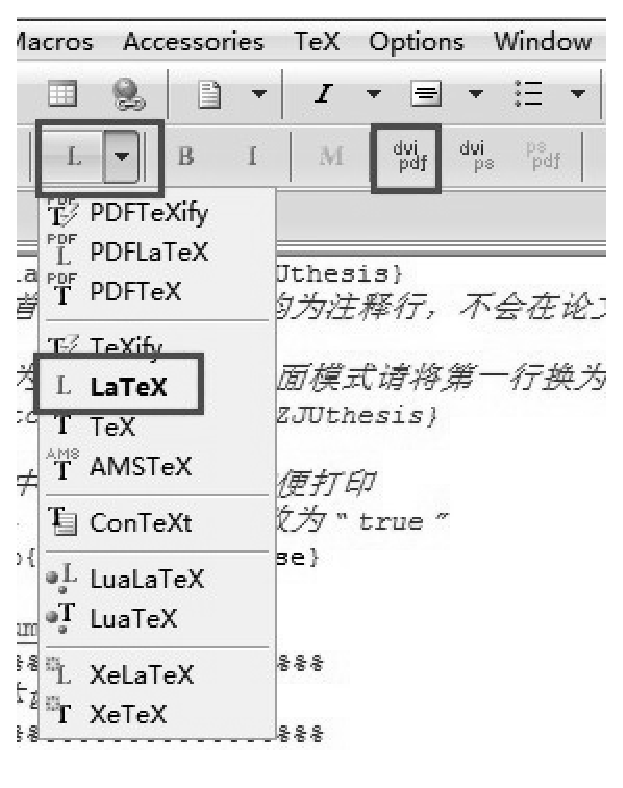
\includegraphics[scale=0.8]{./Pictures/runLaTeX.eps}
\caption{运行LaTeX}
\label{runLaTeX}
\end{figure}

然后点击WinEdt工具栏中的LaTeX命令,大约几秒运行完成后,
再点右边的dvipdf按钮,如图 \ref{runLaTeX} 所示,就可以生成
“LATEX论文模版使用说明.pdf”,打开就可以看到生成的封面了。

点“LaTeX”按钮的时候要注意的是,点右边的小箭头然后在下拉的菜单中只能是选中某个命令,此处选“LaTeX”,
要执行要点到按钮上才行。

还可以创建一个批处理文件来完成这个任务,此处批处理文件内容如下:

%\vspace{4mm}
{\linespread{1}
\zihao{-5}
\begin{verbatim}
latex --src-specials --synctex=-1 LATEX论文模版使用说明
dvipdfmx -p a4 LATEX论文模版使用说明
\end{verbatim}
}
\vspace{4mm}

当前目录下运行这个批处理命令也可以行到“LATEX论文模版使用说明.pdf”文件。

这里要说明的一点是,如果论文中开始加入参考文献,索引等信息,
那么生成pdf文档的流程还要增加,使用WinEdt操作顺序是:先点击“LaTeX”命令按钮,
再点击右边的“B”按钮(生成参考文献信息文件)和“I”按钮(生成索引信息文件);
然后{\bfseries 再}点击“LaTeX”命令{\bfseries 两次},最后再进行dvi到pdf的转换,
否则生成的pdf文件中参考文献与索引的引用处会是“?”号。
如使用批处理命令生成,则相应的批处理文件内容应修改如下:

%\vspace{4mm}
{\linespread{1}
\zihao{-5}
\begin{verbatim}
latex --src-specials --synctex=-1 LATEX论文模版使用说明
makeindex LATEX论文模版使用说明.idx
bibtex LATEX论文模版使用说明
latex --src-specials --synctex=-1 LATEX论文模版使用说明
latex --src-specials --synctex=-1 LATEX论文模版使用说明
dvipdfmx -p a4 LATEX论文模版使用说明
\end{verbatim}
}
\vspace{4mm}

\section{完成题名页信息}

从上节已经完成了封面的信息输入与创建,下面我们进入题名页的创建,
与创建封面页一样,题名页也是先输入信息,再创建页面。

还是回到“论文模版示例.tex”中,
题名页分中文题名页与英文题名页。
创建中文题名页要输入的信息有论文评阅人与答辩委员会名单,
当然,论文在草稿阶段这几个信息是不填的,待到答辩完成,
重新生成论文电子稿时,再填写这些信息。

论文评阅人信息代码及说明如下:

\vspace{8pt}
{
\linespread{1}
\zihao{-5}\noindent
\begin{tabular}{ll}
\verb+\reviewersA{姓\hspace{1em}名\hspace{1.5em}职称\hspace{1.5em}单位}+ & 论文评阅人1\\
\verb+\reviewersB{三字名\hspace{1.5em}职称\hspace{1.5em}单位}+ & 论文评阅人2\\
\verb+\reviewersC{三字名\hspace{1em}三字职\hspace{1em}单位}+ & 论文评阅人3\\
\verb+\reviewersD{姓\hspace{1em}名\hspace{1.5em}职称\hspace{1.5em}单位}+ & 论文评阅人4\\
\verb+\reviewersE{姓\hspace{1em}名\hspace{1.5em}职称\hspace{1.5em}单位}+ & 论文评阅人5\\
\end{tabular}
}
\vspace{8pt}

为了使这部分信息排版美观,这里要注意一点:

规划好“姓名”、“职称”、“单位”所占的空间,单位名称占用空间
尽量不要超过十二个字。
比如:

\begin{center}
\begin{tabular}{l@{:}r}
论文评阅人1
&
\ZJUunderline[220pt]{姓\hspace{1em}名\hspace{1.5em}职称\hspace{1.5em}这个单位名比较长长长}\\
论文评阅人2
&
\ZJUunderline[220pt]{三字名\hspace{1.5em}职称\hspace{1.5em}这个单位名短\hspace{4em}}\\
论文评阅人3
&
\ZJUunderline[220pt]{三字名\hspace{1em}副职称\hspace{1em}这个单位名不很长\hspace{2em}}\\
\end{tabular}
\end{center}

就要比

\begin{center}

\begin{tabular}{l@{:}r}
论文评阅人1
&
\ZJUunderline[220pt]{姓名\hspace{1em}职称\hspace{1em}这个单位名比较长长长}\\
论文评阅人2
&
\ZJUunderline[220pt]{三字名\hspace{1em}职称\hspace{1em}这个单位名短}\\
论文评阅人3
&
\ZJUunderline[220pt]{三字名\hspace{1em}副职称\hspace{1em}这个单位名不很长}\\
\end{tabular}
\end{center}

看起来要好得多。

前者的代码如下:
{\linespread{1}
\zihao{-5}
\begin{verbatim}
\reviewersA{姓\hspace{1em}名\hspace{1.5em}职称\hspace{1.5em}这个单位名比较长长长}
\reviewersB{三字名\hspace{1.5em}职称\hspace{1.5em}这个单位名短\hspace{4em}}
\reviewersC{三字名\hspace{1em}副职称\hspace{1em}这个单位名不和很长\hspace{2em}}
\end{verbatim}
}

注意$\backslash$space{Xem}的用法,一个em就是一个字宽。把所有单位名填充到同一长度,
最长的单位名是10个字,6个字的单位名就要补4个em,8个字的单位名补2个em。
请根据具体情况自行调整。

答辩委员会信息代码及说明如下:

\vspace{8pt}
{
\linespread{1}
\zihao{-5}\noindent
\begin{tabular}{ll}
\verb+\chairman{姓\hspace{1em}名\hspace{1.5em}职称\hspace{1.5em}单位}+ & 答辩委员会主席\\
\verb+\commissionerA{三字名\hspace{1.5em}职称\hspace{1.5em}单位}+ & 答辩委员会成员1\\
\verb+\commissionerB{三字名\hspace{1em}三字职\hspace{1em}单位}+ & 答辩委员会成员2\\
\verb+\commissionerC{姓\hspace{1em}名\hspace{1.5em}职称\hspace{1.5em}单位}+ & 答辩委员会成员3\\
\verb+\commissionerD{姓\hspace{1em}名\hspace{1.5em}职称\hspace{1.5em}单位}+ & 答辩委员会成员4\\
\verb+\commissionerE{姓\hspace{1em}名\hspace{1.5em}职称\hspace{1.5em}单位}+ & 答辩委员会成员5\\
\end{tabular}
}

\vspace{8pt}

答辩委员会信息同样规划好姓名,职称,单位信息,规划方法与评阅人相同。

生成中文题名页

\vspace{8pt}
\verb+\maketitle+
\vspace{8pt}

保存文件,生成PDF预览效果。

英文题名页信息输入与中文题名页类似。

此处英文题名需再输入一次,同样如果一行写不下写成两行。两行分配请自行处理。

{
\linespread{1}
\zihao{-5}\noindent
\begin{tabular}{p{7cm}l}
\verb+\Etitle{English Title}+ & 英文标题\\
\verb+\Etitletl{Second Line}+ & 如果一行写不下,这里写第二行\\
\end{tabular}
}

英文题名页的评阅人与答辩委员会信息及说明如下:

{
\linespread{1}
\zihao{-5}\noindent
\begin{tabular}{ll}
\verb+\EreviewersA{Name\hspace{1.5em}Professional Title\hspace{1.5em}Organization}+ & 论文评阅人1\\
\verb+\EreviewersB{Name\hspace{1.5em}Professional Title\hspace{1.5em}Organization}+ & 论文评阅人2\\
\verb+\EreviewersC{Name\hspace{1.5em}Professional Title\hspace{1.5em}Organization}+ & 论文评阅人3\\
\verb+\EreviewersD{Name\hspace{1.5em}Professional Title\hspace{1.5em}Organization}+ & 论文评阅人4\\
\verb+\EreviewersE{Name\hspace{1.5em}Professional Title\hspace{1.5em}Organization}+ & 论文评阅人5\\
\verb+\Echairman{Name\hspace{1.5em}Professional Title\hspace{1.5em}Organization}+ & 答辩委员会主席\\
\verb+\EcommissionerA{Name\hspace{1.5em}Professional Title\hspace{1.5em}Organization}+ & 答辩委员会成员1\\
\verb+\EcommissionerB{Name\hspace{1.5em}Professional Title\hspace{1.5em}Organization}+ & 答辩委员会成员2\\
\verb+\EcommissionerC{Name\hspace{1.5em}Professional Title\hspace{1.5em}Organization}+ & 答辩委员会成员3\\
\verb+\EcommissionerD{Name\hspace{1.5em}Professional Title\hspace{1.5em}Organization}+ & 答辩委员会成员4\\
\verb+\EcommissionerE{Name\hspace{1.5em}Professional Title\hspace{1.5em}Organization}+ & 答辩委员会成员5\\
\end{tabular}
}

同中文题名页类似,这里的人名,职称,单位信息尽量用简写,否则英文一行可能会写不下。
另外,它们之间的间距请自行设计掌握,与中文信息间距设计方式一致。

至此,英文题名页信息输入完毕。用英文题名页命令生成英文题名页

\vspace{8pt}
\verb+\makeEtitle+
\vspace{8pt}

这里{\bfseries 不要忘记}还有{\bfseries 版权信息页}

{
\zihao{5}
\begin{verbatim}
\SignautreDateA{2013}{10}{11}
\SignautreDateB{2013}{10}{11}
\SignautreDateC{2013}{10}{11}
\makeOSandCPRTpage
\end{verbatim}
}

这里的三个时间命令对应版权信息页中的签字日期信息,
在草稿及送审阶段,这几个命令可以不写。会自动把这几个位置留空。

\section{正文部分各章节的书写}

自此,论文的封面,题名页与版本信息页生成完毕,开始进入论文正文的书写阶段。
下面的内容将不再以命令为主,而是以自己的论文内容为主。

还是回到“论文模版示例”,在正文部分的开始,我们看到这样一个命令:

\verb+\ZJUfrontmatter+

这个命令的意思是开始论文的正文部分,将页码重置为大写罗马数字,并从I开始。


在谈各部分使用之前,写简单谈一下内容部分的书写。
\LaTeX 的文章内容书写没有什么特别的格式,直接书写即可。
但需要注意以下几点:

\begin{enumerate}
\item{\LaTeX 会忽略中文字符间的空格,也就是说:}

{
\linespread{1}
\zihao{-5}
\vspace{8pt}
\noindent\verb+大家好,我的中间没有空格。+\\
{\zihao{-4}和}\\
\verb+大 家 好, 我  的    中   间 没 有 空      格。+
\vspace{8pt}
}

最后输出的内容是一样的。都是:

大家好,我的中间没有空格。

这个“中文字符”包括中文的标点符号,即“。”,“,”等。

如果需要在中文单词间插入空格怎么办?只需要用“\~{}”来代替空格,就像这样:

{
\linespread{1}
\zihao{-5}
\vspace{8pt}
\noindent\verb+大~家~好,~我~的~中~间有很多的空~格。+
\vspace{8pt}
}

这样输出就是这样了:

大~家~好,~我~的~中~间有很多的空~格。

但在英文单词前后的空格,\LaTeX 会{\bfseries 保留一个}。

\item{断行与分段}

\LaTeX 中,{\bfseries 单独一个回车}也会像空格一样被忽略,空行作为分段的标志,
多个连续空行等效于一个空行。此外,还有一个断行命令,
“$\backslash$$\backslash$”,或者是“$\backslash$linebreak”,
这个命令的作用是直接换行但不分段,即新换的行前不空两格。比如

{
\linespread{1}
\zihao{-5}
\vspace{8pt}
我是第一行,\\
我还是第一行。

我是第一段,

我是第二段。

\begin{verbatim}
我是第一行,\\
我是第二行。
\end{verbatim}
\vspace{8pt}
}

出来就是这个效果:

\vspace{8pt}

\hspace{2em}我是第一行,
我还是第一行。

\hspace{2em}我是第一段,

\hspace{2em}我是第二段。

\hspace{2em}我是第一行,\\
我是第二行。

\vspace{8pt}

因此,在编写论文tex文件的时候,同一段落内可以任意换行,
比如写一句话就换一行,这样有利于自己写的时候思路更清晰。
只要不留空行,最后生成的文件都是一整段。

\item{中英文混合编辑时的一个问题及解决方案}

如果某一段文字是中英文字符混合,比如含有单词,
那么如果不做一点特殊处理,\LaTeX 在生成PDF时可能会出现某一行最后一个英文单词突出行外。
解决这个问题的办法就是在英文字符、单词的前面及后面加上空格符号。
当然,这样不太符合我们自己的写作习惯,一个个加起来也太费事。
没关系,\LaTeX 的中文先驱们已经替我们简化了这个问题。
CCT套件中有一个程序:cctspace.exe,只要运行如下格式的命令:

\verb+cctspace [输入文件名] [输出文件名]+

就可以执行这个空格插入操作,而无须手工一个一个添加。

这个程序在安装CTeX环境时已经被安装,可直接使用。使用linux的同学们,请自行在参考文献中的网站中下载源代码编译。

关于这个命令更多的功能选项说明,请参考张林波的《关于新版CCT的说明》\cite{NewCCT:2006}的4.2节部分内容,
很短的,只有一页,纯中文说明文档。


\item{其它的一些要注意的内容}

\LaTeX 中有部分特殊符号不可直接输入,如下:

\verb+#   $   %   ^   &   _   {   }   \+

输入它们要用以下的命令

\verb+\#   \$   \%   \^   \&    \_{}    \{    \}    $\backslash$+

\end{enumerate}

以上就是书写论文正文内容时的一些说明,更多常见问题,请参考《一份不太简短的\LaTeXe 介绍》\cite{LaTeXshzh}和《CTeX FAQ》。
这两个文档都可以在开始--菜单--程序--CTeX--help中找到。


以下将分章节介绍各部分书写时如何使用该模版。

\subsection{勘误页}

其实很少有论文有这样一个部分,但作为一个部分,还是将其做到了模版内。如果不需要,直接将其注释掉或者删除即可。

勘误页的调用命令为

{
\linespread{1}
\zihao{-5}\noindent
\begin{verbatim}
\begin{corrigenda}
这里就写你的勘误内容。
\end{corrigenda}
\end{verbatim}
}

有同学可能会发现,在“论文模版示例.tex”中这部分不是这么写的,我在接下来的致谢介绍中将解释原因。

\subsection{致谢}

致谢的调整命令与勘误页类似,为

{
\linespread{1}
\zihao{-5}\noindent
\begin{verbatim}
\begin{thanks}
这里就写你的致谢内容。
\end{thanks}
\end{verbatim}
}

但是看“论文模版示例.tex”中这一部分却只是简单写了一句:

\verb+\begin{thanks}
在我写这个文档的过程中,得到了网络上很多网贴的帮助,在此感谢baidu,Google,感谢
~CTeX 社区http://www.ctex.org,\LaTeX{}学习园地:http://blog.sina.com.cn/wangzhaoli11,
中科大~CTAN~镜像http://mirrors.ustc.edu.cn/CTAN/,水木社区\TeX{}版等网站、论坛,
其他一些较小的个人网站,论坛不再一一点名,在此一并感谢。
感谢浙江大学数学系提供的原始模版,感谢88\TeX{}版。
\end{thanks}
+

这里的$\backslash$input命令指输入另一个tex文件的内容到当前位置,
就是说\LaTeX 在编译这份tex源文件时读到这里,会去找这里指定的另一个tex文件,
并把它的内容全部复制到这个位置。

这样做的好处是实现了论文的模块化,可以把论文的不现章节写到不同的文件里去,
每个文件都不会太长,更容易查看与修改。在这里这个命令所指向的文件就是当前目录中Chapters目录下的
thanks.tex文件。同学们可以去看一下,这个thanks.tex文件中的内容,是不是就是
跟我上面写的例子是一样的。

要注意的是,这里面的目录名与文件名不能为中文,否则会出错\footnote{linux下的同学可无视这条}。

\subsection{序言}

使用方法同致谢,代码如下:

{
\linespread{1}
\zihao{-5}\noindent
\begin{verbatim}
\begin{preface}
这里就写你的序言的内容。
\end{preface}
\end{verbatim}
}

\subsection{摘要}

摘要的填写与致谢类似,只多了一个关键字命令$\backslash$keywords,具体如下:

{
\linespread{1}
\zihao{-5}\noindent
\begin{verbatim}
\begin{abstractC}
这里就写你的摘要的内容。

\keywords{关健字1,关键字2}
\end{abstractC}
\end{verbatim}
}

\subsection{英文摘要}

英文摘要的填法与中文摘要完全一样,只是都是用英文,具体如下:

{
\linespread{1}
\zihao{-5}\noindent
\begin{verbatim}
\begin{abstractE}
这里就写你的摘要的内容。

\keywordsE{keywords1,keywords2}
\end{abstractC}
\end{verbatim}
}

这个地方要注意的是与中文摘要命令不同之处,abstractE与keywordsE。

\subsection{图片目录}

这一部分只需要如下一个命令,其它的东西\LaTeX 自己会替你搞定。

\verb+\ZJUListofFigures+

如果你不需要图片目录,那么把这条命令删去或者注释掉。

\subsection{表格目录}

这一部分同样只需要如下一个命令,其它的东西\LaTeX 会替你做好。

\verb+\ZJUListofTables+

如果你不需要表格目录,同样只要把这条命令删去或者注释掉即可。

\subsection{缩写、符号清单、术语表}

这一部分与致谢部分相似。代码如下:

{
\linespread{1}
\zihao{-5}\noindent
\begin{verbatim}
\begin{ListofSymbol}
这里就写你的缩写、符号清单、术语表的内容。
\end{ListofSymbol}
\end{verbatim}
}

\subsection{目录}

这一部分只需要如下一个命令,\LaTeX 会替你搞定一切。

\verb+\ZJUcontents+

\subsection{正文章节内容}

到这里,就到了正文章节的编写了。正文部分写法跟致谢,序言的相同,
但致谢,序言没有更小的分节,也不会有图片,表格等内容。
图片,表格方面内容在本说明中放在下面几章中,这里先只介绍正文的章节排布。

在开始正文内容之前,需要一个\LaTeX 命令来告诉软件进入正文部分,
页码需要重新从1编号,并使用阿拉伯数字,以及章节开始从1开始。这个命令是

\verb+\ZJUmainmatter+

正文会有很多章,概述,条件,分析,讨论,结论什么的。编写tex文件的时候,
需要给\LaTeX 明确哪些是章,哪些是节,哪一些是更小的节。这样,\LaTeX 才能正确地给你的正文内容分章,分节

章节标题命令及使用如下:

{
\linespread{1}
\zihao{-5}\noindent
\begin{verbatim}
\chapter{我是章的标题}
我是章标题下的内容
\section{我是第一节的标题}
我是节标题下的内容
\subsection{我是小节的标题}
我是小节的内容。
\begin{enumerate}
\item{我是并列项1}
\item{我是并列项2}
\end{enumerate}
\subsection{我是第二小节的标题}
我是第二小节的内容。
\section{我是第二节的标题}
我是第二节的内容
\subsection{我是第二节第一小节的标题}
我是第二节第一小节的内容
…………
\end{verbatim}
}

章节标题中不需要说明是第几章第几节,\LaTeX 会替你计算,
你所要做的只是把你的文章按结构统一起来即可。
并且,目次也会根据你的标题内容自动生成。
这里要补充一点的是:有的标题可能会比较长,写到目录里会导致目录条目换行,
为解决这个问题,\LaTeX 允许目录中的标题与实际的标题不一样,要达到这个效果,
以章的标题为例,其命令应加一个参数,如下:

\verb+\section[目录中的标题]{实际章节中的标题}+

该模版中章节加上段落可以有6层,足够用了。如表 \ref{ChapsecList} 所示。

\begin{table}[thb]
\zihao{5}
\caption{章节命令}
\label{ChapsecList}
\centering
\begin{minipage}[c]{9cm}
\centering
\begin{tabular}{p{6cm}|c}
\hline
命令 & 层次\\
\hline
\verb+\chapter+ & 章\footnote{实际上在章的上层还有一层叫做part(部分),本模版中用不到。}\\
\hline
\verb+\section+ & 节\\
\hline
\verb+\subsection+ & 小节\\
\hline
\verb+\subsubsection+ & 小小节\\
\hline
\verb+\paragraph+ & 段\\
\hline
\verb+\subparagraph+ & 分段\\
\hline
\end{tabular}
\end{minipage}
\end{table}

另外,如果某处需要用到几个并列项,可以采用enumberate命令,具体代码如下:
{
\linespread{1}
\zihao{-5}\noindent
\begin{verbatim}
  \begin{enumerate}

  \item{我是并列项1} 

  我是并列项1的内容。

  下面将有一个嵌套应用

  \begin{enumerate}
    \item{我是并列项1中的又一个并列项1}

    我是小并列项1的内容。

    \item{我是并列项2中的又一个并列项2}

    我是小并形项2的内容。
  \end{enumerate}

  \item{我是并列项2}

  我是并列项2的内容。

  \end{enumerate}
\end{verbatim}
}

生成文档的效果如下:

\begin{enumerate}
\item{我是并列项1}

我是并列项1的内容。

下面将有一个嵌套应用

\begin{enumerate}
\item{我是并列项1中的又一个并列项1}

我是小并列项1的内容。

\item{我是并列项2中的又一个并列项2}

我是小并形项2的内容。

\end{enumerate}
\item{我是并列项2}

我是并列项2的内容。

\end{enumerate}

\vspace{8pt}

注意tex代码部分中的空行。

这种并列项同样不需要考虑编号问题,\LaTeX 会替你做好一切。
嵌套应用最多可以嵌套三层。

\subsection{参考文献}

正文自此完成了,下面的内容是后面的参考文献,索引,简历等部分。
先需要一个命令告诉软件正文部分结束,开始文后部分

\verb+\ZJUbackmatter+

当正文部分完成后,下一个部分就是参考文献。
参考文献的生成需要准备另外一个参考文献数据文件*.bib,
本说明附带了一个数据文件例子:thesis.bib,
该文件也是一个纯文本文件,可以用记事本打开。
里面给出了七种参考文献的格式:
专利(patent)、标准(standard)、电子文档(Edoc)、
期刊论文(article)、书籍(book)、博/硕士学位论文(mastersthesis/phdthesis)、
其它文献(misc)。

下面以期刊论文为例来说明它的格式。

{
\linespread{1}
\zihao{-5}\noindent
\begin{verbatim}
@article{
LUOZ:2007,
   Author = {罗振 and 田丰 and 孙小平 and 孙恩岩},
   Title = {基于{LATEX}的学位论文模板的设计与实现},
   Journal = {沈阳航空工业学院学报},
   Volume = {24},
   Number = {3},
   Pages = {45-48},
   Year = {2007},
   lang = {chinese}}
\end{verbatim}
}

下面来逐行解释它们表示意义:

@article表示这个文献信息所代表的文献类型是期刊文献。
其它的文献类型见前两段内容。
它后面紧跟的大括号\{\}将这个期刊文献的所有信息括起来。

第二行的“LUOZ:2007”是这个参考文献的引用名,
可以起成任意的方便标识的字符组合,但不能使用中文。
这个字符组合将在文中引用时使用。
以这篇为例,当在论文中使用\verb+\cite{LUOZ:2007}+时,
在生成的文档中此处就会出现引用标号,具体标号\LaTeX 会自己去计算,
后面参考文献部分中的参考文献也由\LaTeX 去排列。
本模版设定的论文引用编号规则是按引用先后排序。

第三行到最后,每一行都代表了该文献的一项信息,
分别是:作者(Author),题目(Title),期刊(Journal),
卷号(Volume),期号(Number),页码(Pages),年份(Year),
语言(lang),每项信息都被\{\}括了起来。要{\bfseries 注意}除了最后一项,
每一项都以一个英文逗号“,”结束;多个作者之间用“and”连接;
如果题目中有连续的大写字母,应用\{\}把它们单独括起来,
如不括起来,除首单词首字母,其它都会被变回小写。

语言的信息项可以不写,这里写上是为了保障对中文文献信息的兼容。

其它几类文献的信息可参考thesis.bib中的填写方法,
与上述说明大同小异。

当所有参考文献信息按thesis.bib中格式填写好,存为一个*.bib文件,
文件名可以任意取,但不能使用中文,比如mybib.bib。

在tex源文件中,只需在文中按上面介绍的$\backslash$cite命令把引用
参考文献的地方一一用标识词标示出来,再在正文的最后使用如下所示的参考文献列表命令,
就可以生成格式完全符合要求的参考文献列表,
这个格式符合要求包括任何一个标点都是正确的!!

\verb+\ZJUthesisbib{mybib}+

请注意这里命令的参数就是你的参数文献数据文件的文件名。


\subsection{附录}

附录以命令\verb+\appendix+开始,随后即可写入附录章节内容。
附录章节内容写法与正文写法完全相同,\LaTeX 会替你处理好章节编号等问题,
你完全不用考虑附录的编号。

{
\linespread{1}
\zihao{-5}\noindent
\begin{verbatim}
\chapter{附录A}
\chapter{附录B}
\end{verbatim}
}

\subsection{索引}

索引与参考文献的使用方法类似,但不需要建立什么数据文件,只要你在文中有索引标记,
到了这里,只需要如下一条命令就能够建立索引。

\verb+\ZJUindex+


\subsection{个人简历}

个人简历部分比较简单,按如下格式书写即可。相信写完论文后,这个完全难不住你们的。

{
\linespread{1}
\zihao{-5}\noindent
\begin{verbatim}
\begin{resume}
\begin{enumerate}
\item{第一条的内容}
\item{第二条内容}
\end{enumerate}
\end{resume}
\end{verbatim}
}

\subsection{发表文章目录}

发表文章目录部分同个人简历部分,命令只是关键字不同。

{
\linespread{1}
\zihao{-5}\noindent
\begin{verbatim}
\begin{publications}
\begin{enumerate}
\item{第一篇}
\item{第二篇}
\end{enumerate}
\end{publications}
\end{verbatim}
}

